\chapter{Multiple Integral} \label{ch7ch}

The integral for scalar input function has been introduced in Chapter \ref{ch3}. The integral of $y=f(x)$ with the lower bound $a$ and upper bound $b$ is denoted by \eqref{ch3eq:generaldefiniteintegral2}. It is defined as the limit of sum given by \eqref{ch3eq:generaldefiniteintegral}, and can be interpreted as the area circulated by $x=a$, $x=b$, $y=f(x)$ and $y=0$ as shown by Fig. \ref{ch3fig:explainintegrial}. In practice, the integral can be calculated using \eqref{ch3eq:calculatedefiniteintegral}.

In this chapter, the integral for multiple input functions is introduced. Motivating examples are used to illustrate the basic concept and meaning of multiple integral in Section \ref{ch7sec:motivatingexp}. The formal definition of multiple integral is given in Section \ref{ch7sec:multipleintegral}.

\section{Motivating Examples} \label{ch7sec:motivatingexp}

\begin{shortbox}
\Boxhead{Motivating Example 1}

Consider calculating the volume of a cone using integral. The bottom radius and the height of the cone are $1$ and $3$ respectively.

\end{shortbox}

Figure \ref{ch7fig:motivatingexp1} gives a demonstration of the cone in the motivating example. Using similar ideas introduced in Chapter \ref{ch3}, we know that we can think of the cone as a combination of thin cylinders, whose radiuses depend on the vertical position ($z$-axis position) of the associated cylinder. For example, at $z=1.5$, the radius of the cylinder is $0.5$.

\begin{figure}
	\centering
	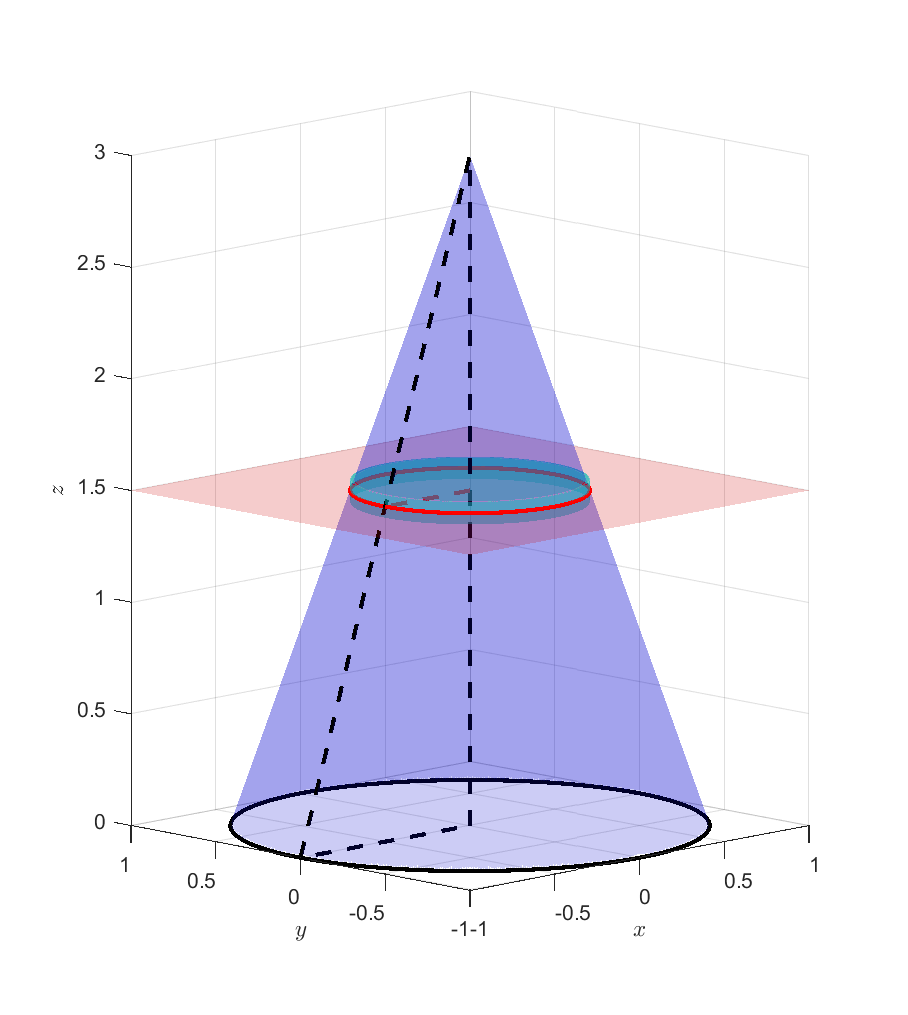
\includegraphics[width=200pt]{chapters/chapter7/figures/motivatingexp1.eps}
	\caption{Calculation of the volume of a cone.} \label{ch7fig:motivatingexp1}
\end{figure}

The volume of the cone can be obtained by letting the thickness of each cylinder approaches zero. i.e.,
\begin{eqnarray}
  V &=& \int_{0}^{3}S(z)dz, \label{ch7eq:motivatingv} \\
  S(z) &=& \pi R(z)^2, \label{ch7eq:motivatingsz} \\
  R(z) &=& \dfrac{3-z}{3}, 0\leq z\leq 3, \label{ch7eq:motivatingrz}
\end{eqnarray}
where $R(z)$ and $S(z)$ are the bottom circle radius and area of the thin cylinder at vertical position $z$, and $S(z)dz$ can be interpreted as the volume of this thin cylinder.

Substituting \eqref{ch7eq:motivatingsz} and \eqref{ch7eq:motivatingrz} into \eqref{ch7eq:motivatingv} gives
\begin{eqnarray}
  V = \int_{0}^{3} \dfrac{\pi}{9} \left(3-z\right)^2 dz
  = \left.\dfrac{\pi}{27}(z-3)^3 \right|_0^3
  = \pi, \nonumber
\end{eqnarray}
which is consistent with what we learned in primary school: the volume of a cone is one third of its bottom area multiplied by its height.

The above motivating example 1 implies the volume of an object might be formulated as an one-dimensional integration. As a first step, a direction, such as $z$-axis as given in the motivating example 1, is chosen. Next, imagine using planes to intersect the object. Each plane shall be perpendicular to the selected direction, as given by the red plane in Fig. \ref{ch7fig:motivatingexp1}. Notice that the red plane is perpendicular to the direction of $z$-axis. The intersection area shall be a function of the intersection position, as given by \eqref{ch7eq:motivatingsz}. Finally, the volume can be calculated as the integral of the area function over the direction, as given by \eqref{ch7eq:motivatingv}.

In many cases, the calculation of the intersection area can be less simple and intuitive than \eqref{ch7eq:motivatingsz}. An example is given by the following motivating example.

\begin{shortbox}
	\Boxhead{Motivating Example 2}
	
	Consider calculating the volume surrounded by the following surfaces:
	\begin{eqnarray}
		0\leq &x& \leq 2\pi, \nonumber \\
		0\leq &y& \leq 2\pi, \nonumber \\
		0\leq &z& \leq f(x,y) = y\textup{cos}(x+y)+2\pi. \label{ch7eq:motivatingexp2f}
	\end{eqnarray}
	
\end{shortbox}

We will use the same method adopted from the motivating example 1 to solve motivating example 2. The volume to be calculated is plotted in Fig. \ref{ch7fig:motivatingexp2} (only the top surface). The $x$-axis direction is chosen for the integral in motivating example 2.

It can be spotted soon that motivating example 2 is more complicated than 1 as the intersection area, in this case $S(x)$ as a function of position $x$, cannot be obtained as intuitively as \eqref{ch7eq:motivatingsz}.

As an example for illustration, in Fig. \ref{ch7fig:motivatingexp2} the red surface is the intersection surface at $x=2$, and $S(x)$ at $x=2$ should be the area surrounded by the red line. At a first glance, it seems that $S(x)$ does not have an analytical expression as the red line shape is quite arbitrary.

\begin{figure}
	\centering
	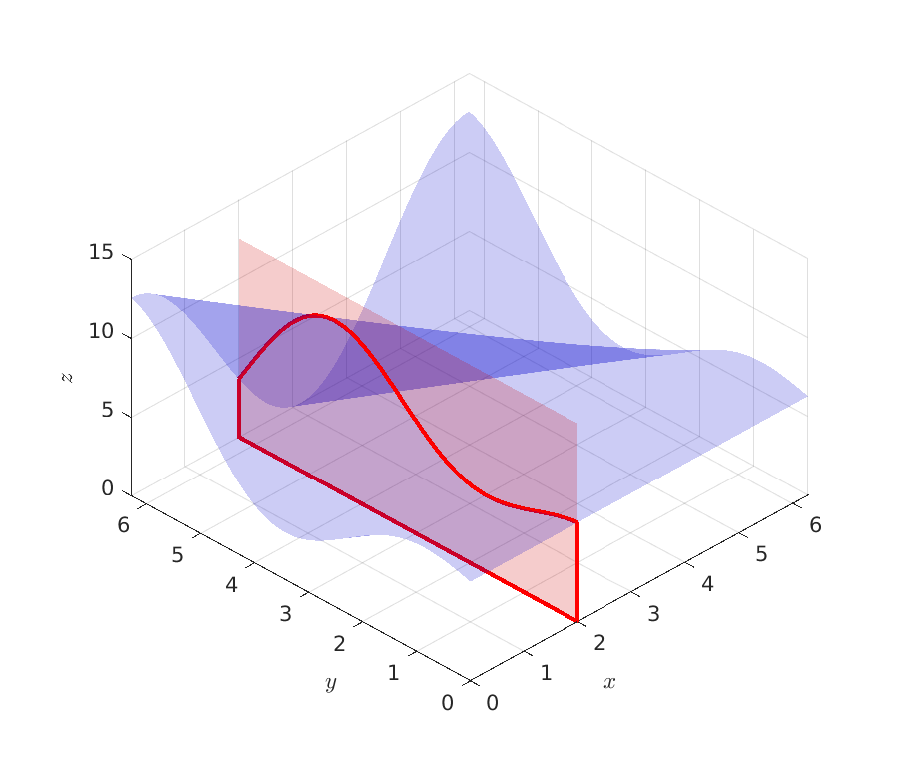
\includegraphics[width=200pt]{chapters/chapter7/figures/motivatingexp2.eps}
	\caption{Calculation of volume of an arbitrary arbitrary project.} \label{ch7fig:motivatingexp2}
\end{figure}

However, this is not true. The area surrounded by the red line in Fig. \ref{ch7fig:motivatingexp2} can be calculated with the knowledge introduced in Chapter \ref{ch3} as follows. Substituting constant $x=2$ into \eqref{ch7eq:motivatingexp2f} gives
\begin{eqnarray}
	z = f(2,y) = y\textup{cos}(y+2) + 2\pi, 0\leq y\leq2\pi, \nonumber
\end{eqnarray}
which is the analytical expression of the red line (intersecting with the top surface). Therefore, the corresponding area in Fig. \ref{ch7fig:motivatingexp2} is
\begin{eqnarray}
	S(x)|_{x=2} &=& \int_{0}^{2\pi} f(2,y) dy \nonumber \\ &=& \int_{0}^{2\pi}\left(y\textup{cos}(y+2) + 2\pi\right)dy \nonumber \\
	&=& \left.\left(y\textup{sin}(y+2)+\textup{cos}(y+2) + 2\pi y\right)\right|_{0}^{2\pi} \nonumber \\
	&=& 2\pi\textup{sin}(2) + 4\pi^2. \nonumber
\end{eqnarray}

Without specifying $x$ as any particular value, $S(x)$ is in general given by
\begin{eqnarray}
	S(x) &=& \int_{0}^{2\pi} f(x,y) dy \label{ch7eq:motivatingexp2sx0} \\ &=& \int_{0}^{2\pi}\left(y\textup{cos}(x+y)+2\pi\right)dy \label{ch7eq:motivatingexp2sx} \\
	&=& \left.\left(y\textup{sin}(x+y)+\textup{cos}(x+y) + 2\pi y\right)\right|_{0}^{2\pi} \label{ch7eq:motivatingexp2sx2} \\
	&=& 2\pi\textup{sin}(x) + 4\pi^2, \label{ch7eq:motivatingexp2sx3}
\end{eqnarray}
where \eqref{ch7eq:motivatingexp2sx2} is derived from \eqref{ch7eq:motivatingexp2sx} by treating $x$ as a constant value. Using  \eqref{ch7eq:motivatingexp2sx0} and \eqref{ch7eq:motivatingexp2sx3}, the volume in motivating example 2 can be calculated as
\begin{eqnarray}
	V &=& \int_{0}^{2\pi} S(x) dx \nonumber \\
	&=& \int_{0}^{2\pi} \left[\int_{0}^{2\pi}f(x,y)dy\right]dx \label{ch7eq:motivatingexp2doubleintegral} \\
	&=& \int_{0}^{2\pi} \left[ \int_{0}^{2\pi}\left(y\textup{cos}(x+y)+2\pi\right)dy\right] dx \nonumber \\
	&=& \int_{0}^{2\pi} \left(2\pi\textup{sin}(x) + 4\pi^2\right) dx \nonumber \\
	&=& \left.\left(-2\pi\textup{cos}(x) + 4\pi^2 x\right)\right|_{0}^{2\pi} \nonumber \\
	&=& 8\pi^3. \nonumber
\end{eqnarray}

In \eqref{ch7eq:motivatingexp2doubleintegral}, two integrals are calculated one after another to finally obtain the volume of motivating example 2. There is an alternative way of understanding \eqref{ch7eq:motivatingexp2doubleintegral} that gives more insights to the problem. From \ref{ch3}, we know that $dx$ and $dy$ are the infinitesimal change along $x$-axis and $y$-axis respectively, and the two-step integrals are essentially the calculation of infinite sum of $f(x,y)$ multiplied by $\Delta x$ and $\Delta y$ as given in the equation below, with $\Delta x, \Delta y \rightarrow 0$. To conclude, \eqref{ch7eq:motivatingexp2doubleintegral} can be rewritten as
\begin{eqnarray}
  \int_{0}^{2\pi} \left[\int_{0}^{2\pi}f(x,y)dy\right]dx &=& \lim_{\Delta x, \Delta y \rightarrow 0} \sum_{i} \left[\sum_{j} f(x_{i},y_{j}) \Delta y \right] \Delta x \nonumber \\
  &=& \lim_{\Delta x, \Delta y \rightarrow 0} \sum_{i,j} f(x_i,y_j) \Delta x \Delta y, \label{ch7eq:motivatingexp2deltaxy}
\end{eqnarray}
where \eqref{ch7eq:motivatingexp2deltaxy} represents the sum of a volume of cubes with the bottom area $\Delta x \times \Delta y$ and different height $f(x_i,y_j)$, as demonstrated by Fig. \ref{ch7fig:motivatingexp2p2}. With $\Delta x, \Delta y \rightarrow 0$, the precise volume of the arbitrary object can be obtained.

\begin{figure}
	\centering
	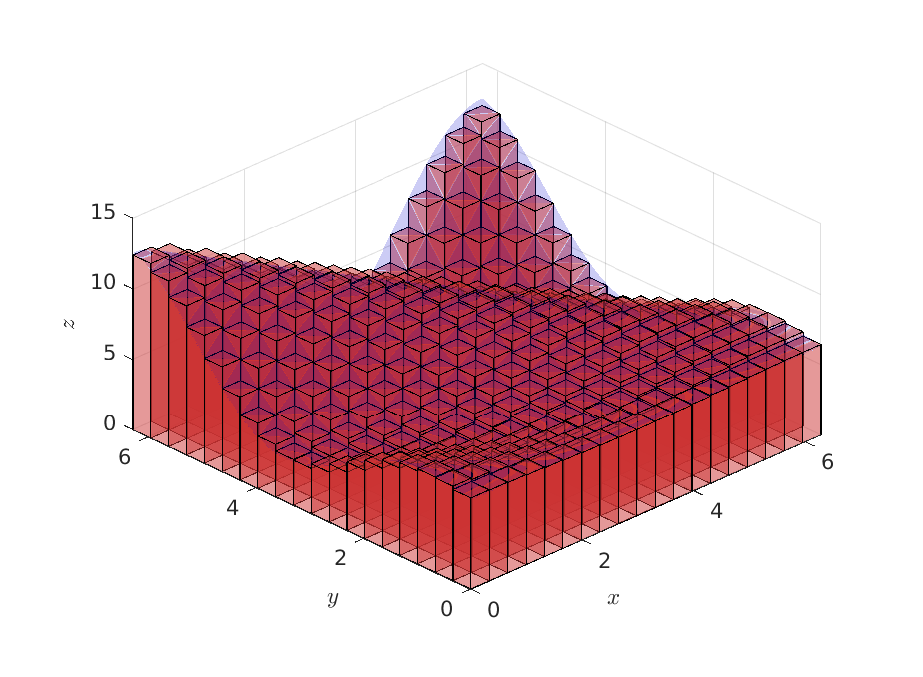
\includegraphics[width=200pt]{chapters/chapter7/figures/motivatingexp2p2.eps}
	\caption{Calculation of volume of an arbitrary object as sum of cubes.} \label{ch7fig:motivatingexp2p2}
\end{figure}

Notice that as long as \eqref{ch7eq:motivatingexp2deltaxy} exists, the sequence of the summation is irrelevant to the result. For example, the cubes with the same $x$-axis position can be added together first (as demonstrated by the red cubes in Fig. \ref{ch7fig:motivatingexp2p3}). Then the sum of volume of cubes at different $x$-axis positions are added together. Similarly, it can be done in the other way around. The cubes with the same $y$-axis position can be added together first (as demonstrated by the green cubes in Fig. \ref{ch7fig:motivatingexp2p3}).

\begin{figure}
	\centering
	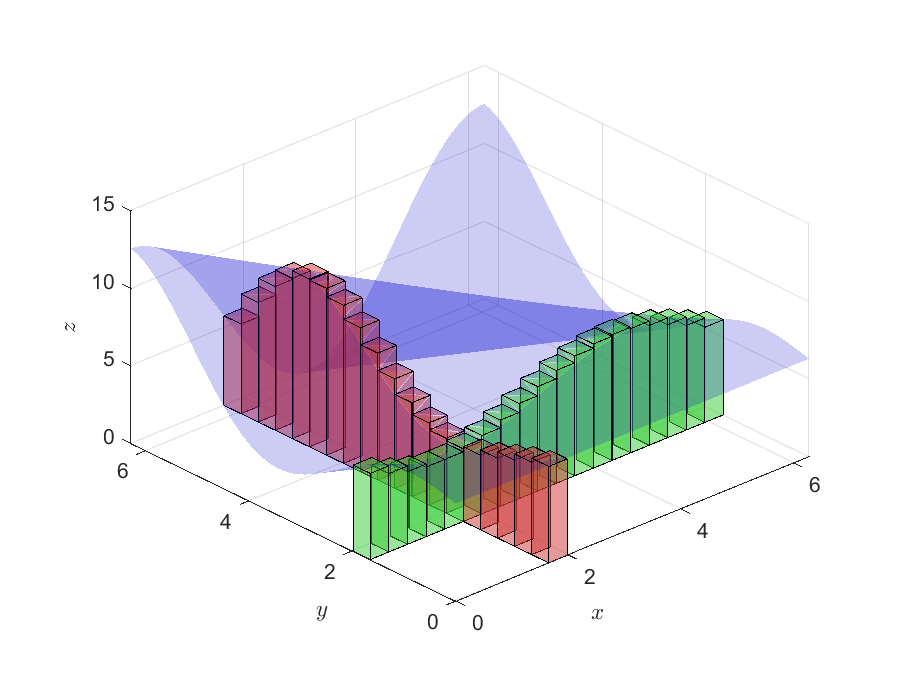
\includegraphics[width=200pt]{chapters/chapter7/figures/motivatingexp2p3.eps}
	\caption{Summation of cubes in different sequence.} \label{ch7fig:motivatingexp2p3}
\end{figure}

Equation \eqref{ch7eq:motivatingexp2deltaxy} is denoted by
\begin{eqnarray}
  \lim_{\Delta x, \Delta y \rightarrow 0} \sum_{i,j} f(x_i,y_j) \Delta x \Delta y &=& \int_{0}^{2\pi}\int_{0}^{2\pi} f(x,y) dx dy ,\label{ch7eq:motivatingexp2def}
\end{eqnarray}
which is an example of double integral. And in this example, we already know that to solve \eqref{ch7eq:motivatingexp2def}, we can use either \eqref{ch7eq:motivatingexp2doubleintegral} or
\begin{eqnarray}
  \int_{0}^{2\pi}\int_{0}^{2\pi} f(x,y) dx dy &=& \int_{0}^{2\pi} \left[\int_{0}^{2\pi}f(x,y)dx\right]dy, \nonumber
\end{eqnarray}
both shall give the same result as the sequence of integral over $x$ or $y$ is irrelevant as long as \eqref{ch7eq:motivatingexp2def} exists. Notice that for multiple integral sometimes $\iint$, $\iiint$, etc., symbols are used for simplicity when the upper and lower boundary of the integral variables are the same or not given in the equation. Thus, \eqref{ch7eq:motivatingexp2def} can also be written as $\iint_{0}^{2\pi} f(x,y)dx dy$.

\section{Multiple Integral} \label{ch7sec:multipleintegral}

The definition of double integral is given below. Higher order of integral can be achieved by expanding the double integral into a higher dimension hyperspace.

\begin{VF}
    \textbf{Definition of Double Integral}:
    \\
    \\
Given a function $f(x,y)$, the double integral of $f$ over the rectangle $R$ is defined by
\begin{eqnarray}
  \iint_{R} f(x,y)dA &=& \lim_{m, n\rightarrow \infty}\sum_{i=1}^{m} \sum_{j=1}^{n} f(x_{ij},y_{ij})\Delta A \label{ch7eq:doubleintegraldef}
\end{eqnarray}
if this limit exists. In \eqref{ch7eq:doubleintegraldef}, $f(x_{ij},y_{ij})$ is an arbitrary sample of $f(x,y)$ in the associated infinitesimal area $\Delta A$.

If $f(x,y)$ is continuous on the rectangle $R = \left\{(x,y)| a\leq x \leq b, c \leq y \leq d \right\}$, then
\begin{eqnarray}
  \iint_{R} f(x,y)dA &=& \iint_{R} f(x,y)dx dy \nonumber \\
  &=& \int_{a}^{b}\int_{c}^{d} f(x,y) dxdy \nonumber \\
  &=& \lim_{m, n\rightarrow \infty}\sum_{i=1}^{m} \sum_{j=1}^{n} f(x_{ij},y_{ij})\Delta x \Delta y \label{ch7eq:doubleintegraldefxy}
\end{eqnarray}

\end{VF}

Equation \eqref{ch7eq:doubleintegraldefxy} can be interpreted as follows. The rectangular is divided into $m\times n$ infinitesimal ``squares'', whose length and width given by $\Delta x$, $\Delta y$ respectively. An example is given in Fig. \ref{ch7fig:motivatingexp2p2} where the bottom of each red cube is such a square. The volume of such a cube is then approximated using $f(x_{ij},y_{ij})\Delta x \Delta y$, where $f(x_{ij},y_{ij})$ is an arbitrary sample of $f(x,y)$ within the associated square. With the populating of the number of cubes, the right side $f(x_{ij},y_{ij})\Delta x \Delta y$ may converge (to the volume between $z=f(x,y)$ and $z=0$ in the given rectangle $R$). If it indeed converges, then the converged value is denoted by the double integral $\iint_{R} f(x,y)dxdy$, where $dxdy$ represents the 2-dimensional infinitesimal square $\Delta x \Delta y$ when they both approach zero.

Equation \eqref{ch7eq:doubleintegraldef} can be expanded to hyperspace for multiple integral with more than 2 variables. In practice, there is no limit to the maximum order of integral in an equation.













